
% Two-pass algorithm, the passes are independent in the
% sense that the can be respectively turned of during a
% cycle.  But not in parallel, due to enumeration-changes
% caused by sharing, unless these changes are kept in a
% mapping.
% 
% First pass, simulation, runs the programs and updates the
% state, calculates new sharing.
% 
% Second pass, geometrication, evaluates shape functions and
% calculates orientation and position based feedback.
% 
% Feedback means coupling the engine with programs, not
% optimal. 
% 
% 
% 
% The sharing of nodes must be found cheaply, since it's
% potentially run very often. Hence comparisons of explicit
% representations of programs, with potential loop
% detection, is probably to expensive.  Instead labelling
% and a few extra operations are used to find applications
% of already evaluated programs.
% 
% We do not want to evaluate programs fully to compare them!
% 
% Sharing may depend on arguments, not only functions, hence
% it's hard to recalculate it fully. 
% 
% Comparison to Fran \& Pan.
% 
% Discrete with interpolation, gives us something simple and
% faithful to our L-system roots while still allowing smooth
% visualisationa.  Also way more efficient than simulating
% more often.
% 
% Implicit monadic structure => extremely simple, easy to
% move functionality between sim.engine and programs.  Once
% the optimal interface is found => move to explicit
% structure, allows better analysis and also compilation to
% lowlevel language. 
% 
% Feedback loop, necessity? Location independence
% compromised?  Global resources (light -> shadows).
% Glob.res. => sim.engine no longer independent of programs.
% Not much to do unless its implementation can be moved to
% the programs, which makes it hard to make nodes sufficient
% independent, where to store the lightbox?
% 
% 
% 
% Conflicts as a result of sharing and hashing, internal
% state not completely hidden. 
% 
% Global resources, account for readings of these, include
% in hashing if used. Or: let a node mark itself as
% independent of a resource. If explicit embedding is used,
% this can be inferred (at least partially).
% 
% 
% A Node. Defines shape, geometry, program. 
% 
% 
% Disallow update of shape?  .. nah
% 
% 
% Suspend until what? Time. Event? 
% 
% It's tempting to move towards event-driven programs, but
% do we really want that?
% 
% What is a step? Program => execute a number of statements
% or react on input?
% 
% 
% Animation, interpolated discrete vs. continuous.
% 
% 
% Possible underlying models, (event, imperative, dna,
% functional, ...) Short discussion and motivation of the
% chosen way.
% 
% 
% Self-similarity on different levels => not shared here.
% 
% 
% Monadic, Leibniz.
% 
%  Weave programs, with shared or individual state.
%
%







\section{Monadic Approach}



    This approach to simulation of plants is heavily influenced by
    Lindenmayer systems described in section \ref{lindenmayer}, but
    with a number of important differences.  As with L-Systems, a
    plant is composed by a number of smaller parts where each part
    grows by either changing its appearance or creating new parts,
    according to a number of rules or instructions.
    However, where an L-System separates the rules from the passive
    symbols, we view them as a single whole, each symbol is extended
    to a unit containing the rules that governs its development.

    This shift in perception, from symbols and rules to
    instruction-containing parts, was the main idea behind this
    approach, with the hope of making it easier both to describe,
    and to combine, high-level behaviours without losing the
    conceptual simplicity of L-Systems.


\begin{figure}[hbt]
    \centering
    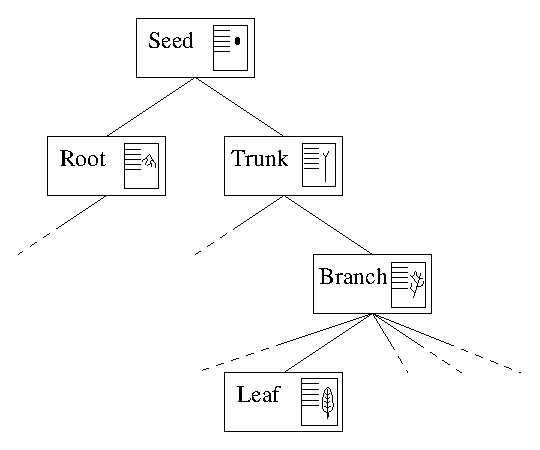
\includegraphics{images/tree_overview}
    \label{monadic:tree_overview}
    \caption{Overview of the internal structure of a simulated tree}
\end{figure}

\subsection{Design Goals}

    A number of design goals lies behind this approach and has guided
    its development, later sections will refer back to these to
    provide motivation for decisions without obvious solutions. These
    are the result both of the initial visions of the system, and much
    experimentation with various simulation cores, given the outlines
    of this approach. Note that they should be seen as guidelines
    rather than rules set in stone, indeed we do break some of them in
    the interest of making something more useful.

\begin{description}
\item[Genericity]
    The core of the simulation engine should be kept generic, without 
    any specific knowledge of things that does not concern its
    functionality, which should be kept minimal. Instead, encode as
    much as possible in the programs in the structure parts.
\item[Independence]
    If parts of a plant only knows very little about each
    other, they are easier to reuse, easier to reason about in
    isolation and it is simpler to discover sharing (see
    section \ref{monadic:sharing}).
\item[Simplicity]
    Only the functionality actually used in a certain part
    should be involved during simulation, no ``dead weight'' or
    default values or programs.
\item[Efficiency] 
    It should be possible to simulate a large number of
    complex plants quickly, preferably in real-time.
    We also want to share representation of similar
    structure parts, this will have lots of consequences for
    the design..

\end{description}

\subsection{Overview}


    A simulated plant is represented as a number of nodes where each
    node corresponds to a major part of the structure of the plant,
    such as a branch or a leaf. The nodes contains all information
    necessary to further their development, visualize them and decide
    when to spawn new subnodes.

    In addition to the actual nodes, which will be dealt with in
    section \ref{monadic:node_internals}, a simulation module and a
    geometry module completes the design. The simulation module
    is responsible for executing the programs in each node, creating
    and destroying nodes upon request and distributing messages. The
    nodes are contained in a tree formed to correspond to their
    relative placement in the plant (see \ref{monadic:tree_overview}). When
    desired, the geometry module traverses the internal structure
    and translates it into a geometrical representation understood by
    the main visualization system (see \ref{system:geomrep}).

    The division in two rather independent passes, simulation and
    geometrification, provides two interesting features:
    When simulating a new world to a given state without
    caring about visualization (until finished), the
    first pass may be run much more often than the
    second, trading accuracy for speed (the visualization
    may be used to calculate feedback originating from
    spatial orientation, which is not directly known in the
    structure tree, more on this in section
    \ref{monadic:feedback}).

    When visualizing a "constant" world (time changing slowly, or not
    at all), the second pass can be used to apply small mutations to
    the model, to give the impression of windy circumstances (rattling
    leaves, bending branches) and also to add detail and
    irregularities.

    The second pass is also used to interpolate between discrete
    states, thus providing smooth animation support cheaply
    (see \ref{monadic:animation}).


\subsubsection{Simulation}

    The simulation code traverses the tree and runs the programs
    associated with the nodes, updating the internal states of all
    nodes and reacting to their behavior. Apart from changing its
    internal state, a node-simulation can have a number of external
    actions: new structure parts may be created, messages can be sent
    to the children or the parent and a node can trigger its own
    death.

    A creation action inserts a new node as a child of the simulated
    part and its program is evaluated once to initialize its state.

    When a part decides to die, itself and all its children are
    removed from the tree.

    Message passing is described in section \ref{monadic:messages}.


\subsubsection{Visualization}

    \label{monadic:viz}

    The shape of a structure part is specified by a function, $ t
    \rightarrow (w \times \mathbf{p}) $, defining the width $w$ and position
    $\mathbf{p}$ along its length $[0..t]$. The parameter $t$ is
    initialized to zero upon creation and the program in each node is
    responsible for updating it according to its development.
    But shape alone is not enough to generally visualize a plant, the
    exact geometry which should be generated must also be specified,
    and this is done by a function parameterized over both the
    parameter $t$ and the shape-function: $ t \rightarrow
    (t \rightarrow (w \times \mathbf{p})) \rightarrow
    [\mathit{geometry}] $. A number of geometric primitives are
    available, such as cylinders, cones and splines (for branches) and
    textured surfaces (for leaves). These are further described in
    section \ref{system:geomrep} and the set of primitives can quite
    easily be extended to allow modelling of more complex parts
    (flowers, for example). 
 
    These three components are stored in each node and may be updated
    during its development, but the shape and geometry functions are
    usually only assigned once upon creation. The presentation above
    is slightly simplified, in addition to the parameter $t$ the
    functions may refer both to the internal state of a node and its
    orientation, the former to allow the shape to depend on more than
    a single parameter and the latter be able to take gravitation into
    account. 

    The complete geometrical representation of a plant is simply
    generated by traversing all nodes and collecting geometry from
    each one of them, using $\mathit{shape}$ functions to get the
    relative placement between the resulting structure parts.


    This model may seem unnecessary complex, why not just have a
    single function returning geometric representation directly:
    ($ \mathit{node} \rightarrow [\mathit{geometry}] $)? 
    The introduced complications can be argued for as follows:
\begin{itemize}
\item We must know where to place subnodes on a node, this could be
        done by storing the exact coodinates but this has the disadvantage
        that they must be fixed for the whole life-time of a part
        unless a possibility to update them is available. Instead,
        each subnode stores the value of the parameter $t$ which was
        current when it was created, and when we need to place a
        subnode we just apply the $\mathit{shape}$-function to it.
        This keeps all shape-related functionality in one place.

\item Subnodes should be placed on the
        surface of the parent, not in the center, thus we need to know the
        width along a nodes extension (think of placing leaves on a branch).

\item Orientation is not known during simulation, but we do want to
        take it into account (bending branches due to gravitation),
        thus we need this as a parameter as well (a vector pointing
        down, in the nodes local coordinate system, is actually
        enough) and this is provided during generation of geometry.
        Note that it is actually impossible to know the orientation
        during simulation if we also want to share nodes (see
        \ref{monadic:sharing}), because a single node may have several
        parents and thus several orientations at once!

\end{itemize}


    A number of convenience functions are available, making
    specification of appearance much simpler than the above
    description may give the impression of.


\subsection{Node Internals}

\label{monadic:node_internals}

    A node manages, in addition to the parameters describes in the
    preceding section, its program and an internal state which can be
    updated and queried by the program. The programs are constructed
    by combining a number of core operations, either sequentially or
    in parallel. Normally a specific behaviour is coded as a sequence
    of operations and several aspects of a plant's behaviour are
    combined together in parallel.

    The operations are described by small example programs, to give a
    feel for how they are used rather than just specifying syntax.
    Note that the language is not very stable at the moment, details
    may change.


\subsubsection{Core Operations}

    The power of this approach lies in the possibility to build
    libraries of higher level operations out of the quite small number
    of primitive operations described in this section. 

\paragraph{Appearance}

    The components described in section \ref{monadic:viz} can be
    assigned by the following instructions:

\begin{haskell*}
branch = \hsdooo{
        shape (\fn{t}{(0.1, {\bf e}_y `scaled\!\_\!by` t)}) \\
        geometry (mk\!\_\!branch brown) \\
        set\!\_\!pos 1}
\end{haskell*}
The above program specifies a brown branch, following the
y-coordinate axis, with a constant length of one.

Not very interesting though, it doesn't grow. To do that we need to
update the position each step.

\begin{haskell*}
init\!\_\!branch = \hsdooo{
    shape (\fn{t}{(0.1, {\bf e}_y `scaled\!\_\!by` t)}) \\
    geometry (mk\!\_\!branch brown)} \\
grow\!\_\!by g = \hsdooo{ 
        p \hsfrom get\!\_\!pos \\
        set\_pos (p\!+\!g) }\\
branch = \hsdooo{
    init\!\_\!branch \\
    loop (grow\!\_\!by \ 0.1) } \\
\end{haskell*}

The \emph{loop} function runs its argument over and over again,
until \emph{stop} is encountered.
\begin{haskell*}
branch = \hsdooo{
        init\!\_\!branch \\
        loop \$ \hsdoo{
            grow\!\_\!by \ 0.2 \\
            p \hsfrom get\_pos \\
            when (p\!>\!1) stop
        }}
\end{haskell*}

    We have already seen a number of interesting properties of the
    language, thanks to being embedded in haskell we get a lot for
    free, especially the ability to abstract out common functionality
    in reusable functions.


\paragraph{Spawning}

    To create substructures the functions \emph{spawn} and
    \emph{spawn\_ori} are used, the former keeps the orientation
    of the parent while the latter allows arbitrary rotations to be
    applied.

\begin{haskell*}
leaf = \hsdooo{
    shape (\fn{t}{(t,{\bf e}_y})) \\
    geometry (mk\uc{}leaf (texture ``green\_leaf'')) \\
    loop (get\uc{}pos >\!\!>\!\!= set\uc{}pos . min 1 . (+0.2)) \\
} \\
branch = \hsdooo{
    init\!\_\!branch \\
    loop \$ \hsdoo{
        grow\!\_\!by \ 0.5 \\
        spawn\!\_\!ori \ ({\bf e}_z `rotate` (pi/3)) \ leaf \\
        grow\!\_\!by \ 0.5 \\
        spawn\!\_\!ori \ ({\bf e}_z `rotate` (-pi/3)) \ leaf \\
  }                    
}
\end{haskell*}

This program grows a branch which spawns a green leaf every 0.5 units
of its length, on alternating sides.

\paragraph{Message propagation}

\label{monadic:messages}

    Nodes may interchange messages (currently only strings)
    to propagate resources or signals either upwards or downwards in
    the node hierarchy. One example of usage is to signal leaves to
    fall off synchronized when the parent-branch has run out of
    energy. Messages should only be used when no other options are
    available, they don't fit very well in the model and was only
    added because some problems cannot be solved without them, in an
    acceptably simple way.


\paragraph{Parallelism}

    As mentioned in the introduction to this section programs may be
    combined in parallel as well as sequentially. This turned out to
    be a very powerful abstraction mechanism since it allows different
    behaviours to be encoded as individual and independent program
    fragments.

\begin{haskell*}
stop\uc{}at \ p_{max} = \hsdooo{
    p \hsfrom get\uc{}pos \\
    when (p >= p_{max}) stop
} \\
branch = \hsalg{
    init\uc{}branch \ `weave` \\
    \quad loop (grow\uc{}by \ 0.2 \ `weave` \ stop\uc{}at \ 1.0)\\
 }
\end{haskell*}

    The function \emph{weave} combines two program fragments by
    returning running each of them one step further every time itself
    is run, thus weaving them together.

    But how long is a step? Since the simulation is discrete we must
    have a way to determine how many instructions to run in each
    program each time its node is simulated. This is done by the
    instruction \emph{suspend}, which saves the current state and 
    triggers the execution of the next program in turn.
    Thus \emph{loop} could be implemented as:

\begin{haskell*}
loop m = \hsdooo{
    m \\
    suspend \\
    loop m \\
}
\end{haskell*}

    It is not done this way, due to reasons related to sharing of
    nodes, but it can be thought of the above program in all essential
    ways.
    An alternative to an explicit \emph{suspend} function would be to
    suspend after every instruction, but that would result in
    unnecessary inefficient execution with only a slight syntactic
    gain. And it could be problematic to get a feel for how fast
    different program executes relative to each other.

\paragraph{Local State}

    An arbitrary number of parameters can be stored in the internal
    state for each node, these can be used to implement new operations
    for behaviours not possible with the provided single length
    parameter, for example keeping track of resource levels, mass or
    growth parameters.


\subsubsection{Gravitation}

    To calculate gravitational effects we need to know some
    things we have not considered yet, the density and
    elasticity of a branch and its orientation. The density
    and elasticity can be stored in the internal state and
    the orientation is made available to us by the visualization
    module. Essentially, the shape function is adapted to take these
    effects into account using an sufficently advanced model regarding
    the desired effects. It is worth noting that one can get very far
    with very simple models, appendix \ref{monadic_examples} contains
    a few examples of this.


\subsubsection{Forests}

    The language can not only be used to describe single plants, but
    also groupings of them. Instead of starting with a branch with
    spawns other brances and leaves we start with a meta-node, which
    in turns spawns whole plants places as usual with its
    shape-function (which now defines the surface of the
    forest-covered area).
    To avoid symmetrical and repetetive patterns random numbers should
    be used when placing plants and determining their types.


\subsubsection{L-system simulation}


\label{lsystem_to_dsel}

    Traditional L-system can be simulated by creating one node-type
    for each symbol, containing the parameters for parametric
    L-systems. The rewrite-rules are rewritten as programs which
    updates the state accordingly and spawns new subnodes when
    the corresponding rule would trigger such action.
    
    The plants in figure \ref{param-lsys-example} are generated using 
    the following program, taken from an example in
    \cite{lsys_theory_vis}:

\newpage
\begin{haskell*}
lsystem = \hsdooo{
       geometry (mk\uc{}branch (Flat (0.2, 0.6, 0.15))) \\
       st \hsfrom getst \\
       shape (\fn{t}{(max (w st) 0.01, (down `scaled\uc{}by` 0.6t) + (0,2t,0))}) \\
       loop \$ \hsdooo{ 
         LSys \alpha_1 \alpha_2 \varphi_1 \varphi_2 w_0 min_s r_1 r_2 q s w cs \hsfrom getst \\
         \hscase{(cs < s, s <= min_s)}{\\
          \!\!(\_, True) \ra stop \\
          (True, \_) \ra \hsdoo{
               modst (\fn{s}{s \{ cs = cs + 0.02 \}}) \\
               set\uc{}pos cs 
          } \\
          \_ \ra \hsdooo{
             set\uc{}pos s \\
	     \hskwd{let} new\uc{}child \alpha \varphi r q = spawn\uc{}ori \\\hspace{8mm}\hsidnt{
                            ({\bf e}_z `rotate` \alpha `mulq` {\bf e}_y `rotate` \varphi) \\
                            (\hsdoo{ modst (\fn{p}{initial\uc{}state
                            \{ s=r\!\cdot\!s, w=q\!\cdot\!w \})} \\
                                next plant\uc{}lsystem) }}\\
             new\uc{}child \alpha_1 \varphi_1 r_1 q \\
             new\uc{}child \alpha_2 \varphi_2 r_2 (1\!-\!q) \\
             stop }
         }
       }
 }
\end{haskell*}
    The sequence \emph{next f} is a shorthand for \emph{suspend} followed by
    \emph{f}, \emph{mulq} combines two rotation operations.

    Here we also see the usage of \emph{getst} and \emph{modst} to
    operate on the local state, which type is defined as a usual
    haskell data-type not shown here. An alternative, and simpler,
    interface to the local state is also available, which avoids the
    need to define a new data-type.

    Context sensitive L-system are a bit harder to
    simulate, since the only inter-node mechanism available is
    message-passing each rewrite has to be rewritten as a
    number of steps which first query the surroundings and
    then change node accordingly, no work has been made in
    this area.



\subsection{Feedback}

\label{monadic:feedback}

    During simulation the internal nodes are completely agnostic of
    location and orientation, however sometimes we do want to add
    dependencies on global properties such as sunlight, shadows and
    global resource levels.
    This bookkeeping could be done in an extra pass between
    geometry-generation (the only time when we know absolute positions
    and orientations) and the next simulation pass, by calculating
    appropriate feedback and apply to nodes requesting it.
    (this is work-in-progress.)

\subsection{Animation}

\label{monadic:animation}

    Since this approach uses a simulation algorithm with discrete
    steps, smooth animation it not possible out-of-the-box. However,
    the representation of geometric information has been carefully
    chosen to allow interpolation between states, which allows us
    arbitrary precision of animations without involving the simulation
    algorithm at all. Best results are achieved if the
    programs are written with animation in mind, since the (linear)
    interpolation only works well for small changes in appearance. 


\subsection{Sharing}

\label{monadic:sharing}


    For a tree with, for example, a couple of thousands leaves, it is
    very wasteful to represent and simulate each one of them
    individually, it is quite probable that a large number of them
    will be in a equal or similar state of development at any given
    point in time. To take advantage of this, the simulation algorithm
    tries to find equal or mostly equal structures and merge them,
    thus only simulating and representing them once. This greatly
    improves the performance of big scenes but also put a lot of
    limitations on the implementation, to find sharable parts we have
    to compare the nodes for equality, which is a bit challenging
    since they both contain computations and state of arbitrary types
    (functions, for example, are not comparable in haskell). 

    Two techniques are used to work around this limitation, one is to
    encode functions using an explicit notation as abstract
    expression trees, and another is to use an impure ``hack'' similar
    to the one Koen Claessen uses to discover sharing in circuit
    descriptions in \cite{obs_sharing}.  The former is used for
    shape-functions and the latter for node-programs. This solution is
    not completely satisfactory since it fails to discover some
    opportunities for sharing, but it is just an optimization so the
    only consequence is a slightly slower simulation. This is one
    price we have to pay for using an embedded language in Haskell, we
    do not have access to the concrete programs, only the expressions
    they generates, thus obvious shared references in the
    text-representation of programs are not visibile to us, but
    have to be rediscovered.

    An alternative would be to use an explicit notation also for
    programs, but since they can be quite long, and have to be
    compared often (potentially each simulation step), it was
    considered as a bad tradeoff even if more opportunities to sharing
    would arise. 

